\ifx\allfiles\undefined
\documentclass[8pt a4paper, oneside, UTF8]{ctexbook} 
\usepackage{amsmath}   % 数学公式
\usepackage[dvipsnames]{xcolor}
\usepackage{amsthm}    % 定理环境
\usepackage{amssymb}   % 更多公式符号
\usepackage{graphicx}  % 插图
\usepackage{mathrsfs}  % 数学字体
\usepackage{enumitem}  % 列表
\usepackage{geometry}  % 页面调整
\usepackage{unicode-math}
\usepackage{extarrows}
\usepackage{subfigure}
\usepackage{extarrows}
\usepackage{footnote}
\usepackage{svg}
\usepackage[colorlinks,linkcolor=black]{hyperref}
\usepackage{supertabular}
\usepackage{tcolorbox}
\usepackage{ulem}
\usepackage{framed}
\usepackage{float}
\usepackage{microtype}
\newcommand{\arccot}{\mathrm{arccot}\,}
\tcbuselibrary{breakable}
\tcbuselibrary{most}
\newcounter{problemname}
\newenvironment{solution}{\par\noindent\textbf{解答. }}{\par}
\newenvironment{note}{\par\noindent\textbf{题目\arabic{problemname}的注记. }}{\par}
\definecolor{shadecolor}{RGB}{241, 241, 255}
\newenvironment{problem}{\begin{shaded}\stepcounter{problemname}\par\noindent\textbf{题目\arabic{problemname}. }}{\end{shaded}\par}

\graphicspath{ {figure/},{../figure/}, {config/}, {../config/} }  % 配置图形文件检索目录
\linespread{1.2} % 行高

% 页码设置
\geometry{top=25.4mm,bottom=25.4mm,left=20mm,right=20mm,headheight=2.17cm,headsep=4mm,footskip=12mm}

% 设置列表环境的上下间距
\setenumerate[1]{itemsep=5pt,partopsep=0pt,parsep=\parskip,topsep=5pt}
\setitemize[1]{itemsep=5pt,partopsep=0pt,parsep=\parskip,topsep=5pt}
\setdescription{itemsep=5pt,partopsep=0pt,parsep=\parskip,topsep=5pt}

% 定理环境
% ########## 定理环境 start ####################################

% #### 将 config.tex 中的定理环境的对应部分替换为如下内容
% 定义单独编号,其他四个共用一个编号计数 这里只列举了五种,其他可类似定义(未定义的使用原来的也可)
\newtcbtheorem[auto counter, number within=section, list type=subsubsection, list inside=toc]{defn}{定义}
{
    colback=green!5,colframe=green!35!black,fonttitle=\bfseries, title={Comment \thetcbcounter}, list entry={Comment \thetcbcounter\quad}, %标题
    breakable, %支持跨页
    before upper={\parindent10pt\noindent},  % 支持缩进。\noindent:首行不缩进
    % left = 2mm, %文字离线框左边的边距
    % right = 1mm,%同上
    % top = 1mm,%同上
    % bottom = 1mm,%同上
    % arc is angular = 1mm, % 棱角线框
    % sharp corners, % 直角线框
    % enhanced,frame hidden, % 隐藏线框
    % enhanced, drop fuzzy shadow,  % 显示阴影
}
{def}

\newtcbtheorem[auto counter, number within=section, list type=subsubsection, list inside=toc]{lemma}{引理}
{
    colback=SeaGreen!10!CornflowerBlue!10,colframe=RoyalPurple!55!Aquamarine!100!,fonttitle=\bfseries, title={Comment \thetcbcounter}, list entry={Comment \thetcbcounter\quad}, %标题
    breakable, %支持跨页
    before upper={\parindent10pt\noindent},  % 支持缩进。\noindent:首行不缩进
    % left = 2mm, %文字离线框左边的边距
    % right = 1mm,%同上
    % top = 1mm,%同上
    % bottom = 1mm,%同上
    % arc is angular = 1mm, % 棱角线框
    % sharp corners, % 直角线框
    % enhanced,frame hidden, % 隐藏线框
    % enhanced, drop fuzzy shadow,  % 显示阴影
}
{lem}


\newtcbtheorem[auto counter, number within=section, list type=subsubsection, list inside=toc]{them}{定理}
{
    colback=Salmon!20, colframe=Salmon!90!Black,fonttitle=\bfseries, title={Comment \thetcbcounter}, list entry={Comment \thetcbcounter\quad}, %标题
    breakable, %支持跨页
    before upper={\parindent10pt\noindent},  % 支持缩进。\noindent:首行不缩进
    % left = 2mm, %文字离线框左边的边距
    % right = 1mm,%同上
    % top = 1mm,%同上
    % bottom = 1mm,%同上
    % arc is angular = 1mm, % 棱角线框
    % sharp corners, % 直角线框
    % enhanced,frame hidden, % 隐藏线框
    % enhanced, drop fuzzy shadow,  % 显示阴影
}
{them}
\newtcbtheorem[auto counter, number within=section, list type=subsubsection, list inside=toc]{criterion}{注}
{
    colback=CornflowerBlue!10,colframe=RoyalPurple!55!Aquamarine!100!,fonttitle=\bfseries, title={Comment \thetcbcounter}, list entry={Comment \thetcbcounter\quad}, %标题
    breakable, %支持跨页
    before upper={\parindent10pt\noindent},  % 支持缩进。\noindent:首行不缩进
    % left = 2mm, %文字离线框左边的边距
    % right = 1mm,%同上
    % top = 1mm,%同上
    % bottom = 1mm,%同上
    % arc is angular = 1mm, % 棱角线框
    % sharp corners, % 直角线框
    % enhanced,frame hidden, % 隐藏线框
    % enhanced, drop fuzzy shadow,  % 显示阴影
}
{cri}

\newtcbtheorem[auto counter, number within=section, list type=subsubsection, list inside=toc]{corollary}{推论}
{
    colback=Emerald!10,colframe=cyan!40!black,fonttitle=\bfseries, title={Comment \thetcbcounter}, list entry={Comment \thetcbcounter\quad}, %标题
    breakable, %支持跨页
    before upper={\parindent10pt\noindent},  % 支持缩进。\noindent:首行不缩进
    % left = 2mm, %文字离线框左边的边距
    % right = 1mm,%同上
    % top = 1mm,%同上
    % bottom = 1mm,%同上
    % arc is angular = 1mm, % 棱角线框
    % sharp corners, % 直角线框
    % enhanced,frame hidden, % 隐藏线框
    % enhanced, drop fuzzy shadow,  % 显示阴影
}
{cor}
% colback=red!5,colframe=red!75!black

% ######### 定理环境 end  #####################################

% ↓↓↓↓↓↓↓↓↓↓↓↓↓↓↓↓↓ 以下是自定义的命令  ↓↓↓↓↓↓↓↓↓↓↓↓↓↓↓↓

% 用于调整表格的高度  使用 \hline\xrowht{25pt}
\newcommand{\xrowht}[2][0]{\addstackgap[.5\dimexpr#2\relax]{\vphantom{#1}}}

% 表格环境内长内容换行  
\newcommand{\tabincell}[2]{\begin{tabular}{@{}#1@{}}#2\end{tabular}}

% 使用\linespread{1.5} 之后 cases 环境的行高也会改变,重新定义一个 ca 环境可以自动控制 cases 环境行高
\newenvironment{ca}[1][1]{\linespread{#1} \selectfont \begin{cases}}{\end{cases}}
% 和上面一样
\newenvironment{vx}[1][1]{\linespread{#1} \selectfont \begin{vmatrix}}{\end{vmatrix}}

\def\d{\textup{d}} % 直立体 d 用于微分符号 dx
\def\R{\mathbb{R}} % 实数域
\newcommand{\bs}[1]{\boldsymbol{#1}}    % 加粗,常用于向量
\newcommand{\ora}[1]{\overrightarrow{#1}} % 向量

% 数学 平行 符号
\newcommand{\pll}{\kern 0.5em/\kern -0.8em /\kern 0.5em}

% 用于空行\myspace{1} 表示空一行 填 2 表示空两行  
\newcommand{\myspace}[1]{\par\vspace{#1\baselineskip}}

\begin{document}
\begin{sloppypar}
    % \title{{\Huge{\textbf{高等数学笔记}}}}
\author{作者:于家崇}
\date{\today}
\maketitle                   % 在单独的标题页上生成一个标题

\thispagestyle{empty}        % 前言页面不使用页码
\begin{center}
	\Huge\textbf{前言}
\end{center}

If a job is worth doing,it's worth doing well
\begin{flushright}
	\begin{tabular}{c}
		\today \\ 如果一件事值得去做,那就值得去做好
	\end{tabular}
\end{flushright}

\newpage                      % 新的一页
\pagestyle{plain}             % 设置页眉和页脚的排版方式(plain:页眉是空的,页脚只包含一个居中的页码)
\setcounter{page}{1}          % 重新定义页码从第一页开始
\pagenumbering{Roman}         % 使用大写的罗马数字作为页码
\tableofcontents              % 生成目录

\newpage                      % 以下是正文
\pagestyle{plain}
\setcounter{page}{1}          % 使用阿拉伯数字作为页码
\pagenumbering{arabic}
% \setcounter{chapter}{-1}    % 设置 -1 可作为第零章绪论从第零章开始 
    \else
    \fi
    %  ############################ 正文部分
    \chapter{连续}
    \section{函数的连续性}
    \begin{defn}{连续点的定义}{}
        设函数$y=f(x)$在点$x_0$的某一邻域内有定义,如果
        $$
            \lim_{x\to x_0}f(x)=f(x_0)
        $$
        那就称为函数$y=f(x)$在点$x_0$连续.
    \end{defn}
    \begin{criterion}{函数连续的性质}{}
        \begin{itemize}
            \item 当极限需要讨论时:
            $$
            \lim_{x\to x_0^+}f\left(x\right)=\lim_{x\to x_0^-}f\left(x\right)=f\left(x_0\right)\Leftrightarrow f\left(x\right)\text{ 在点 }x_0\text{ 处连续}
            $$
            \item 连续性的四则运算:设$f(x)$与$g(x)$都在点$x=x_0$处连续,则$f(x)\pm g(x)$与$f(x)g(x)$在点$x=x_{0}$处连续,当$g(x_0)\neq0$ 时,$f(x)/g(x)$在点$x=x_{0}$处也连续。
            \item 复合函数的连续性:设$u=\varphi(x)$在点$x=x_0$处连续,$y=f(u)$在点$u=u_0$处连续,且$u_{0}=\varphi(x_{0})$,则$f\left[\varphi(x)\right]$在点$x=x_{0}$处连续。
            \item 反函数的连续性:设$y=f(x)$在区间$I_x$上单调且连续,则反函数$x=\varphi(y)$在对应的区间 $I_{y}=\{y|y=f(x),x\in I_{x}\}$ 上连续且有相同的单调性
            \item \textbf{$f(x)$在点$x=x_0$处连续,且$f(x_0)>0$(或$f(x_0)<0$),则存在$\delta>0$,使得当$|x-x_0|<\delta$时 $f\left(x\right)>0\left(\text{或}f\left(x\right)<0\right).$ }
        \end{itemize}
    \end{criterion}
    \section{函数的间断点}
    \subsection{间断点的相关概念}
    \begin{defn}{}{}
        可去间断点:若$\lim_{x\to x_0}f(x)=A\neq f(x_0)(f(x_0)$甚至可以无定义),则这类间断点称为可去间断点
        \begin{center}
            \tikzset{every picture/.style={line width=0.75pt}} %set default line width to 0.75pt        
            \begin{tikzpicture}[x=0.75pt,y=0.75pt,yscale=-1,xscale=1]
            \draw  (151,148.43) -- (349.86,148.43)(250.09,67.87) -- (250.09,231.3) (342.86,143.43) -- (349.86,148.43) -- (342.86,153.43) (245.09,74.87) -- (250.09,67.87) -- (255.09,74.87) (270.09,143.43) -- (270.09,153.43)(290.09,143.43) -- (290.09,153.43)(310.09,143.43) -- (310.09,153.43)(330.09,143.43) -- (330.09,153.43)(230.09,143.43) -- (230.09,153.43)(210.09,143.43) -- (210.09,153.43)(190.09,143.43) -- (190.09,153.43)(170.09,143.43) -- (170.09,153.43)(245.09,128.43) -- (255.09,128.43)(245.09,108.43) -- (255.09,108.43)(245.09,88.43) -- (255.09,88.43)(245.09,168.43) -- (255.09,168.43)(245.09,188.43) -- (255.09,188.43)(245.09,208.43) -- (255.09,208.43) ;
            \draw   ;
            \draw    (250.09,148.43) -- (313.36,62.43) ;
            \draw   (297,81.43) .. controls (297,80.13) and (298.06,79.07) .. (299.36,79.07) .. controls (300.66,79.07) and (301.71,80.13) .. (301.71,81.43) .. controls (301.71,82.73) and (300.66,83.79) .. (299.36,83.79) .. controls (298.06,83.79) and (297,82.73) .. (297,81.43) -- cycle ;
            \draw  [fill={rgb, 255:red, 0; green, 0; blue, 0 }  ,fill opacity=1 ] (298.64,147.57) .. controls (298.64,146.55) and (299.47,145.71) .. (300.5,145.71) .. controls (301.53,145.71) and (302.36,146.55) .. (302.36,147.57) .. controls (302.36,148.6) and (301.53,149.43) .. (300.5,149.43) .. controls (299.47,149.43) and (298.64,148.6) .. (298.64,147.57) -- cycle ;
            \draw (246,43) node [anchor=north west][inner sep=0.75pt]   [align=left] {$\displaystyle y$};
            \draw (353,138) node [anchor=north west][inner sep=0.75pt]   [align=left] {$\displaystyle x$};
            \draw (233,149) node [anchor=north west][inner sep=0.75pt]   [align=left] {$\displaystyle O$};
            \draw (122,138) node [anchor=north west][inner sep=0.75pt]   [align=left] {$ $};
            \draw (181,236) node [anchor=north west][inner sep=0.75pt]   [align=left] {可去间断点函数图像};
            \end{tikzpicture}            
        \end{center}
    \end{defn}
    \begin{defn}{}{}
        跳跃间断点\footnote{一点极限存在\neq f(x)在$x_0$连续}:若$\lim_{x\to x_0^-}f(x)$与$\lim_{x\to x_0^+}f(x)$都存在,但$\lim_{x\to x_0^+}f(x)\neq\lim_{x\to x_0^-}f(x)$,则这类间断点称为跳跃间断点
        \begin{center}
            \tikzset{every picture/.style={line width=0.75pt}} %set default line width to 0.75pt        
            \begin{tikzpicture}[x=0.75pt,y=0.75pt,yscale=-1,xscale=1]
            \draw  (152.86,148.43) -- (351.71,148.43)(251.95,67.87) -- (251.95,231.3) (344.71,143.43) -- (351.71,148.43) -- (344.71,153.43) (246.95,74.87) -- (251.95,67.87) -- (256.95,74.87) (271.95,143.43) -- (271.95,153.43)(291.95,143.43) -- (291.95,153.43)(311.95,143.43) -- (311.95,153.43)(331.95,143.43) -- (331.95,153.43)(231.95,143.43) -- (231.95,153.43)(211.95,143.43) -- (211.95,153.43)(191.95,143.43) -- (191.95,153.43)(171.95,143.43) -- (171.95,153.43)(246.95,128.43) -- (256.95,128.43)(246.95,108.43) -- (256.95,108.43)(246.95,88.43) -- (256.95,88.43)(246.95,168.43) -- (256.95,168.43)(246.95,188.43) -- (256.95,188.43)(246.95,208.43) -- (256.95,208.43) ;
            \draw   ;
            \draw    (250.09,108.43) -- (352.36,109.43) ;
            \draw   (250.09,108.43) .. controls (250.09,107.13) and (251.15,106.07) .. (252.45,106.07) .. controls (253.75,106.07) and (254.81,107.13) .. (254.81,108.43) .. controls (254.81,109.73) and (253.75,110.79) .. (252.45,110.79) .. controls (251.15,110.79) and (250.09,109.73) .. (250.09,108.43) -- cycle ;
            \draw  [fill={rgb, 255:red, 0; green, 0; blue, 0 }  ,fill opacity=1 ] (250.09,148.43) .. controls (250.09,147.4) and (250.92,146.57) .. (251.95,146.57) .. controls (252.97,146.57) and (253.81,147.4) .. (253.81,148.43) .. controls (253.81,149.45) and (252.97,150.29) .. (251.95,150.29) .. controls (250.92,150.29) and (250.09,149.45) .. (250.09,148.43) -- cycle ;
            \draw    (150.09,187.43) -- (252.36,188.43) ;
            \draw   (250,188.43) .. controls (250,187.13) and (251.06,186.07) .. (252.36,186.07) .. controls (253.66,186.07) and (254.71,187.13) .. (254.71,188.43) .. controls (254.71,189.73) and (253.66,190.79) .. (252.36,190.79) .. controls (251.06,190.79) and (250,189.73) .. (250,188.43) -- cycle ;
            \draw (246,43) node [anchor=north west][inner sep=0.75pt]   [align=left] {$\displaystyle y$};
            \draw (353,138) node [anchor=north west][inner sep=0.75pt]   [align=left] {$\displaystyle x$};
            \draw (233,149) node [anchor=north west][inner sep=0.75pt]   [align=left] {$\displaystyle O$};
            \draw (122,138) node [anchor=north west][inner sep=0.75pt]   [align=left] {$ $};
            \draw (181,236) node [anchor=north west][inner sep=0.75pt]   [align=left] {跳跃间断点函数图像};
            \end{tikzpicture}
        \end{center}
    \end{defn}
    \begin{defn}{}{}
        无穷间断点:若$\lim_{x\to x_0}f(x)=\infty$,则这类间断点称为无穷间断点,如$y=\tan x$
              \begin{figure}[H]
                  \centering 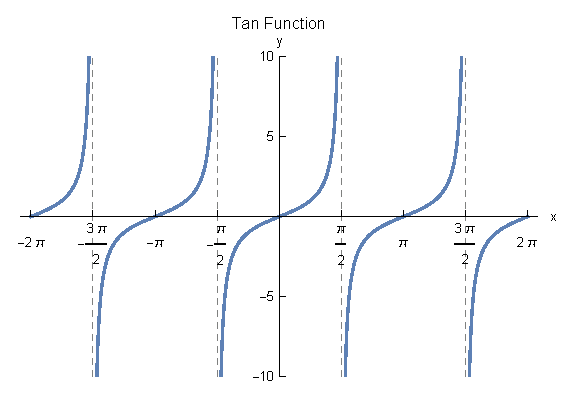
\includegraphics[width=
                      0.4 \linewidth]{1.3.6.eps} \caption{无穷间断点函数tan图像}
              \end{figure}
    \end{defn}
    \begin{defn}{}{}
        振荡间断点:若$\lim_{x\to x_0}f(x)$振荡不存在,则这类间断点称为振荡间断点
              \begin{figure}[H]
                  \centering 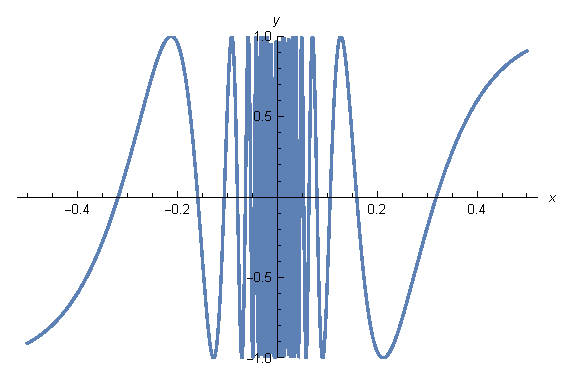
\includegraphics[width=
                      0.4 \linewidth]{3.2.3.eps} \caption{振荡间断点函数$\sin \frac{1}{x}$图像}
              \end{figure}
    \end{defn}    
    \subsection{间断点的分类}
    通过求函数在该点的左右极限来判断
    \begin{itemize}
        \item 第一类间断点:$\lim _ { x \rightarrow x _ { 0 } ^{-}} f ( x )$​ 和$\lim _ { x \rightarrow x _ { 0 }^ {+}} f ( x )$​ 均存在
              \begin{itemize}
                  \item 可去\footnote{可去间断点上极限存在但是导数不存在}:$\lim _ { x \rightarrow x_0 ^ { - } } f ( x ) = \lim _ { x \rightarrow x_0^{+} } f  ( x ) \neq f(x_0)$
                  \item 跳跃:$\lim _ { x \rightarrow x_0^{-} } f ( x ) \not= \lim _ { x \rightarrow x_0^{+} } f ( x )$
              \end{itemize}
        \item 第二类间断点:除第一类以外的间断点$\implies \lim _ { x \rightarrow x _ { 0 } ^{-}} f ( x )$和$\lim _ { x \rightarrow x _ { 0 }^ {+}} f ( x )$​ 均至少一个不存在
    \end{itemize}
    %  ############################ 正文部分
    \ifx\allfiles\undefined
\end{sloppypar}
\end{document}
\fi
